% !TEX program = xelatex
\documentclass[preprint,12pt]{elsarticle}

\usepackage{graphicx}
\usepackage{booktabs}
\usepackage{amsmath,amssymb}
\usepackage{siunitx}
\usepackage[hidelinks]{hyperref}
\usepackage{xcolor}
\usepackage{multirow}
\usepackage{threeparttable}

% 草稿期标注：定稿前应全部清除（用 grep -n torefresh 检查）
\newcommand{\torefresh}[1]{\textcolor{red}{[#1]}}

\journal{Empirical Software Engineering}

\begin{document}

\begin{frontmatter}

\title{Identifiability and Confounding in Test-Adequacy Metric Validity Studies:
A Cross-Language Empirical Analysis}

\author[a]{Anonymous Author(s)}
\affiliation[a]{Anonymous Institution}

\begin{abstract}
A large body of software engineering research asks whether a test-adequacy
metric predicts a suite's ability to detect real faults. The standard
argument regresses a fault-detection outcome on existing metrics, adds the
candidate metric, and interprets the cross-validated $R^2$ gain and its
significance as evidence of incremental value. This paper asks whether that
evidence can be statistically resolved at the sample sizes the literature
uses. We construct test-suite subsets on two independent benchmarks---Defects4J
(Java) and BugsInPy (Python), seven projects each---derive each subset's
fault-detection rate from per-fault trigger-test metadata without executing
the suites, and quantify the uncertainty of the incremental $R^2$ under
several defensible evaluation schemes. We report four findings. (i)~The
incremental $R^2$ of a behavioural-matching feature block has a 95\%
interval width of \num{0.062} on Defects4J and \num{0.143} on BugsInPy under version-level resampling, and \num{0.129} and \num{0.146} respectively under a project-level cluster bootstrap that treats whole projects as the independent units; the sign of the effect is not stable across evaluation schemes on Defects4J. (ii)~A parameterised simulation calibrated on the observed data
shows that when a feature has zero within-project effect but its project
means correlate with baseline detection rates, an unadjusted pooled
analysis reports a non-trivial increment in up to 94\% of runs, whereas
project fixed effects reduce this below 1\%. (iii)~Behavioural features
identify the source project with \num{0.876} and \num{0.824} accuracy against a uniform-random-guess baseline of $1/7 \approx \num{0.143}$, on Java and Python respectively, and the same holds when the classifier is evaluated on held-out fault versions;
project-mean independence is not achieved by any feature family tested.
(iv)~Our resolution curves suggest that attaining a \num{0.05} target
half-width under the project-level bootstrap needs on the order of $70$
independent fault versions, and a \num{0.02} target needs on the order of
$100$. We conclude that incremental-validity claims at the
magnitudes common in this literature are not identifiable at conventional
sample sizes, and we provide a pre-submission protocol---independent-unit count,
size, project discriminability, fixed-effect replication, and resolution
reporting---together with the resolution curves needed to size a study
before it is run.
\end{abstract}

\begin{keyword}
test adequacy \sep fault detection \sep empirical software engineering \sep
validity \sep replication \sep statistical resolution
\end{keyword}

\end{frontmatter}

% =====================================================================
\section{Introduction}
\label{sec:intro}

Software engineering research has produced a large family of test-adequacy
metrics: statement and branch coverage, mutation score, checked coverage,
oracle gap, pseudo-tested methods, semantic coverage, and behavioural
verification gaps, among others. For each of them the central validity
question is the same: \emph{does the metric carry information about whether a
test suite will detect real faults, beyond what simpler and cheaper metrics
already provide?}

The prevailing way to answer this question is incremental-prediction
analysis. A fault-detection outcome is regressed on a baseline set of
metrics, the candidate metric is added, and the resulting gain in explained
variance---usually reported as an increment in $R^2$, or as the coefficient
and $p$-value of the added predictor---is interpreted as evidence of
incremental value.

This paper asks a prior question: \emph{is that evidence statistically
resolvable at the sample sizes the literature uses?} We use
\emph{resolvable} (and, interchangeably, \emph{identifiable at the design
level}) in an operational rather than a causal-inference sense: an
incremental effect is resolvable when the uncertainty of the estimated
increment, together with its sensitivity to defensible analysis choices, is
small relative to the effect magnitude the study claims to have
established. Two properties of the setting make the answer non-obvious.

\textbf{First, the units of analysis are not independent.} A study that
draws many test suites from a small number of subject programs, or many
subsets from each of a few fault versions, accumulates nominal sample size
without accumulating independent information. Significance tests computed
over nominal instances overstate precision, and cluster resampling can change the intervals
substantially---in our data, by a factor of about two on Defects4J.

\textbf{Second, project identity is a strong common cause.} Style, size,
coverage instrumentation, and fault composition all vary systematically
across subject programs, and so do the distributions of almost any derived
metric. A metric that merely distinguishes projects will appear to predict
fault detection in any pooled analysis, even if it has no effect within any
project.

Neither concern is exotic, and both are discussed in the statistical
literature. What is missing is a quantitative account of how much they
matter for the specific claims this community makes. This paper supplies
that account, and it does so on two benchmarks in two languages with a
common outcome construction.

\paragraph{Contributions}
\begin{enumerate}
\item \textbf{A resolution analysis of incremental-validity claims}
(Section~\ref{sec:rq1}). On two benchmarks we show that the incremental
$R^2$ of a behavioural-matching feature block is of the same order as its
own uncertainty, that its sign on Defects4J depends on the cross-validation
scheme, and---using resolution curves---how many independent fault versions a study needs in order to resolve effects of
\num{0.10}, \num{0.05}, and \num{0.02}.
\item \textbf{A mechanism and its rate} (Section~\ref{sec:rq2}). A
simulation calibrated on the observed data isolates project-level
confounding as a driver, and measures the rate at which the unadjusted
analysis reports an increment as a function of confounding strength $\rho$
and sample size. Because $\rho$ is directly estimable from project-level
means, the sensitivity analysis is cheap.
\item \textbf{A cross-language replication} (Section~\ref{sec:rq3}). The
project-fingerprint phenomenon appears on both Defects4J (Java) and
BugsInPy (Python), with identical random baselines, and the pooled analysis
favours the larger model on both.
\item \textbf{A robustness analysis over analytic choices}
(Section~\ref{sec:rq4}). Leave-one-project-out, removal of the dominant
project, project-size thresholds, and two bootstrap hierarchies, each
reported with the effect on the conclusion.
\item \textbf{A pre-submission protocol} (Section~\ref{sec:protocol}) with
five checks, none of which requires executing the test suites under study.
\end{enumerate}

% =====================================================================
\section{Background and Related Work}
\label{sec:related}

\subsection{Test-adequacy metrics and their validity}

Coverage-based metrics are the oldest and most widely used. Inozemtseva and
Holmes \cite{inozemtseva2014coverage} studied the correlation between
coverage and fault detection over 31{,}000 test suites and five real faults,
and found the correlation to be weak and strongly conditioned on suite size;
the result has been a touchstone for the claim that coverage is an
insufficient measure of test quality. Mutation score was argued to be a
better predictor by Papadakis et al.\ \cite{papadakis2018mutation}, who
analysed correlation with real fault detection under controlled conditions
and carefully separated masking effects from genuine detection.

A second family measures what the tests actually \emph{check}. Checked
coverage \cite{schuler2011checked} measures the fraction of covered
statements that influence an assertion through the dynamic slice.
Pseudo-tested methods \cite{niedermayr2016pseudo} identify methods whose
bodies can be deleted without any test failing; Vera-P{\'e}rez et al.\
\cite{vera2019comprehensive} replicated the phenomenon at scale. The
``oracle gap'' \cite{jain2023mindthegap} contrasts coverage with mutation
score to locate oracle weaknesses. Semantic coverage
\cite{ayad2025detecting} measures failure-revealing capability directly, and
Paul and Holmes \cite{paul2026beyond} extract expected behaviours from
documentation and source and measure how many are never verified by any
test.

These works are the immediate context for ours. Two shared features matter
here: their validity arguments are frequently explanatory rather than
predictive---the metric is argued to capture something meaningful, rather
than being shown to predict fault detection at a stated confidence
level---and they are rarely compared with each other under a common
outcome variable. Our contribution is orthogonal: we do not propose a new
metric, but examine whether the inferential machinery used to validate
metrics can support the conclusions drawn from it.

\subsection{Statistical practice in multi-project empirical studies}

The concerns we quantify are instances of long-standing issues in applied
statistics. Non-independence of observations drawn from clusters motivates
cluster-robust standard errors and mixed-effects models
\cite{liang1986longitudinal}; in the software engineering literature these
are standard tools \cite{briand2000recapture} but are applied unevenly.
Confounding by group identity is the setting of Simpson's paradox
\cite{simpson1951interpretation}, and the fixed-effects estimator that
removes it is textbook econometrics \cite{wooldridge2010econometric}.
Publication and reporting practice---in particular the tendency to report
point estimates and $p$-values without interval width or a
minimum-detectable-effect statement---is the subject of a broad
meta-scientific literature \cite{ioannidis2005contamination}; the specific
recommendation we arrive at, that a study state the smallest effect its
design could have detected, is the standard power-analysis requirement
\cite{cohen1988statistical} applied in the mode of sensitivity analysis
\cite{hoenig2001abuse}.

Our contribution is not the introduction of these tools but their
calibration for this community's claims: we measure the magnitudes, on real
benchmarks, and show that at conventional sample sizes the corrected
comparison cannot resolve the effects being claimed. We also show that the
choice of resampling unit---individual fault versions or whole
projects---changes the reported uncertainty substantially, which is a
practical matter rarely addressed in this literature.

\paragraph{Hierarchical structure, clustered inference, and effective
sample size} Observations in this setting are nested---subsets within
fault versions within projects---and the nesting is not incidental: it
determines how much independent information a study actually contains.
Cluster-robust inference \cite{liang1986longitudinal} and effective-sample-size
adjustments are the standard responses, and grouped (``leave-group-out'')
cross-validation is the analogous correction at the model-selection stage:
randomly splitting nested observations leaks group-level information into
the test folds and yields optimistically biased estimates of out-of-sample
performance \cite{roberts2017crossvalidation}. We use grouped
cross-validation throughout for this reason, and report both instance-level
and version-grouped versions of the project-classification diagnostic to
show the difference it makes in our setting.

\paragraph{Fixed effects versus random effects} Group identity can be
handled either by fixed effects, which estimate a separate intercept per
group and identify the effect purely from within-group variation, or by
random effects, which model the group intercepts as draws from a
distribution and can in principle recover between-group information
\cite{wooldridge2010econometric}. We use fixed effects because the
question we ask is explicitly within-project---whether a metric helps
discriminate suites of the same project---and because with seven groups
the random-effects variance components would themselves be poorly
determined.

\paragraph{The bootstrap with few clusters} Cluster resampling is
unreliable when the number of clusters is small, and the resulting
intervals can be too narrow rather than too wide
\cite{cameron2008bootstrap}. With seven projects per benchmark our
project-level intervals fall squarely in that regime, which is why we
present them as a sensitivity analysis rather than as calibrated
confidence intervals, and why we report the version-level hierarchy
alongside them rather than choosing one.

\paragraph{Project heterogeneity in empirical software engineering} The
statistical points above are not new to software engineering practice, even
if their magnitudes for metric-validity claims are not usually measured.
Cross-project and within-project analyses are known to produce different
answers: cost-estimation studies show systematic differences between
cross-company and within-company models \cite{kitchenham2007cross}, and
cross-project defect prediction degrades sharply when the source and target
projects differ in domain or process \cite{zimmermann2009cross}, with
process and organisational factors explaining as much as code metrics
\cite{nagappan2006mining}. Our contribution is to quantify the analogous
effect for test-adequacy metrics, and to show that in this setting the
within-project comparison cannot resolve the effects being claimed.

\subsection{Benchmarks}

Defects4J \cite{just2014defects4j} provides real Java faults with
per-fault trigger tests, which makes a fault-detection outcome computable
without executing the suites under study. BugsInPy
\cite{widyasari2020bugsinpy} provides the analogous Python resource: each
fault records the single test that triggers it. The availability of trigger
metadata in both benchmarks is what makes a common outcome variable
possible across languages.

% =====================================================================
\section{Study Design}
\label{sec:design}

\subsection{Unit of analysis}

The unit is a \emph{test-suite subset}: a fraction of a project's test suite
at a specific fault version. Varying the fraction gives within-version
variation in suite size and in composition, which is what the incremental
analysis requires. Independent information, however, accumulates at the
level of fault \emph{versions}, not subsets, and we report both the nominal
sample size and the number of independent fault-version units throughout.
We use the latter as a count of independent units rather than as a formal
effective sample size (Section~\ref{sec:protocol}).

\subsection{Benchmarks and subjects}

We use seven projects from each benchmark (Table~\ref{tab:subjects}). On
Defects4J we measure on the \emph{fixed} version of each fault, because
mutation analysis aborts on versions whose trigger tests fail; on BugsInPy
we likewise use the fixed version so that the suite pool is well defined.
All analyses are therefore about suite variation at a stable program
revision, not about the fault itself.

\begin{table}[t]
\centering
\begin{threeparttable}
\caption{Analysis sample. A \emph{version} is a \texttt{(project, fault)}
pair with at least one usable subset; an \emph{instance} is one subset run.
Counts are those that enter the analysis, after dropping records with
incomplete metric measurement (Defects4J: \num{3} of \num{302} instances;
BugsInPy: \num{1} of \num{246}).}
\label{tab:subjects}
\begin{tabular}{llrrr}
\toprule
Benchmark & Project & Versions & Instances & Mean line coverage (\%) \\
\midrule
\multirow{7}{*}{Defects4J}
 & Chart    & 14 &  49 & 27.4 \\
 & Cli      &  6 &  12 & 49.4 \\
 & Codec    &  5 &  10 & 23.3 \\
 & Compress & 16 &  29 & 36.1 \\
 & Csv      &  5 &   7 & 50.3 \\
 & Lang     & 34 & 124 & 31.7 \\
 & Math     & 32 &  68 & 33.2 \\
\midrule
\multirow{7}{*}{BugsInPy}
 & black      & 18 &  54 & 83.1 \\
 & fastapi    &  3 &   9 & 86.0 \\
 & httpie     &  2 &   6 & 77.0 \\
 & sanic      &  1 &   3 & 71.3 \\
 & tornado    &  6 &  17 & 38.1 \\
 & tqdm       &  9 &  27 & 70.3 \\
 & youtube-dl & 43 & 129 & 29.1 \\
\bottomrule
\end{tabular}
\begin{tablenotes}\footnotesize
\item The version counts differ from the number of faults available in each
project: they are the versions for which a usable subset could be
constructed. Coverage of either benchmark is therefore partial. On
Defects4J the analysed versions span the seven projects listed; the
remaining ten Defects4J projects were not collected. On BugsInPy, the
usable versions per project range from \num{1} (sanic) to \num{43}
(youtube-dl).
\end{tablenotes}
\end{threeparttable}
\end{table}

\subsection{Constructing subsets}
\label{sec:subsets}

Defects4J's coverage and mutation commands do not accept an explicit test
list, and the framework rewrites \texttt{all\_tests}. We therefore exploit
the fact that each project's build files define the test sources with a
fileset over the \emph{test source directory}: moving the sources of
non-selected tests out of that directory causes the framework to build and
run only the selected subset. Two details were necessary in practice:
(i)~test classes reference each other, so the selected set must be closed
under a dependency closure; (ii)~aggregating test classes
(e.g.\ \texttt{*PackageTests}) are compiled even when not run, so failure
to restore them breaks the build. We restore missing sources adaptively by
parsing \texttt{javac}'s missing-symbol errors and copying the named
classes back from a staging area, iterating until compilation succeeds.

On BugsInPy, subsets are far simpler: \texttt{pytest} accepts an explicit
list of test node identifiers, so no source relocation is needed. The pool
for a version is the set of collected tests that pass at the fixed revision.

\subsection{Outcome variable: differential fault detection}

For a subset $S$ of project $P$'s test suite, the outcome is
\begin{equation}
\mathrm{detect}(S) \;=\;
\frac{\bigl|\{\, f \in \mathcal{F}_P \;:\; \mathrm{trigger}(f) \in S \,\}\bigr|}
     {\bigl|\mathcal{F}_P\bigr|},
\end{equation}
where $\mathcal{F}_P$ is the set of faults of $P$ and
$\mathrm{trigger}(f)$ is the test recorded as triggering fault $f$. The
outcome is computed purely from metadata: \emph{no suite under study is
executed to obtain it}. This avoids executing the suites under study and makes the outcome deterministic and cheap to compute, but it does \emph{not} eliminate the clean-program assumption inherent in trigger-test-based fault detection \cite{chekam2017empirical}: the metadata records which test the fault's patch makes fail, not whether a passing suite would have revealed the fault.

Two calibration details apply. On BugsInPy, trigger tests are occasionally
declared on a \texttt{unittest} base class that \texttt{pytest} does not
collect directly (only its subclasses); we therefore match triggers at the
level of (file, method name) and restrict $\mathcal{F}_P$ to faults whose
trigger falls inside the runnable pool---otherwise faults carried by
network-dependent tests would depress the outcome systematically.

\subsection{Predictors}

\begin{itemize}
\item \textbf{Size}: $\log$ of the number of tests actually run.
\item \textbf{Coverage}: line coverage of the project's own sources
(Defects4J: all main classes instrumented; BugsInPy: the project package
plus top-level modules).
\item \textbf{Mutation score}: Defects4J only, measured on a paired sample
of \num{15} classes per version for cost reasons. BugsInPy has no
comparable low-cost mutation toolchain, so the classical block there is
size $+$ coverage.
\item \textbf{Behavioural matching} (the candidate block): assertion-level
features---assertions per test method, ratio of strong to weak assertions,
ratio of predicate-form assertions, and distinct calls per assertion. These
are syntactic proxies for the semantic notion of ``the test asserts what
the code is supposed to do''.
\end{itemize}

\subsection{Analysis}

We compare four nested models: size; the classical block; size $+$
behaviour; and all predictors. Comparisons use $K$-fold cross-validation
\emph{grouped by fault version}, so that no version contributes to both
training and test folds. We report the result with and without project
fixed effects, and, as a sensitivity check on the fold construction, under
leave-one-version-out cross-validation.

Uncertainty is estimated by bootstrap. Because the choice of resampling
unit is consequential and rarely stated in this literature, we report
\emph{two} hierarchies throughout: resampling individual fault versions,
and resampling whole projects as clusters. The second reflects a more conservative dependence structure, treating projects rather than fault versions as the independent resampling units; with only seven projects per benchmark it is also the more variable estimator, and we interpret it as a sensitivity analysis rather than as a definitive frequentist confidence interval.

\paragraph{Estimator for the cross-validated $R^2$} Throughout we report
the pooled (nested) form
\begin{equation}
R^2_{\mathrm{CV}} \;=\;
1 - \frac{\sum_{i=1}^{n}\bigl(y_i - \hat{y}_{i,\,-g(i)}\bigr)^2}
        {\sum_{i=1}^{n}\bigl(y_i - \bar{y}\bigr)^2},
\end{equation}
where $g(i)$ is the fault version of observation $i$,
$\hat{y}_{i,-g(i)}$ is its prediction from the model fitted on all folds
except the one holding out $g(i)$, and $\bar{y}$ is the grand mean. We do
not average per-fold $R^2$ values, which can be dominated by folds with
little outcome variance and are not comparable across resamples.

\paragraph{Bootstrap specification} Each replicate resamples units with
replacement---fault versions for the version-level hierarchy, whole
projects for the project-level one---and recomputes $\Delta R^2$ on the
resampled data using the same grouped $K$-fold scheme, with folds
recomputed within each replicate. Intervals are percentile intervals from $B = 2000$ replicates, so that each tail of the 95\% interval is supported by about 50 replicates rather than the handful that $B=200$ would provide; the resolution curves in Table~\ref{tab:mde} use $B = 1000$ replicates per point. we also report the fraction of replicates in which
$\Delta R^2 \le 0$. Replicates yielding fewer than six versions are
discarded: six is the smallest number for which the grouped five-fold
cross-validation used in every comparison is defined. Point estimates and bootstrap means are reported separately:
the former is the statistic computed on the full sample, the latter the
mean of the resampling distribution, and they need not coincide. With only
seven project clusters per benchmark, the project-level intervals are
themselves imprecisely estimated; the project-level bootstrap is therefore
used to expose sensitivity to the assumed independent unit, not to claim a
well-calibrated seven-cluster confidence interval.

% =====================================================================
\section{RQ1: To what extent can incremental-validity effects be resolved
at realistic sample sizes?}
\label{sec:rq1}

\subsection{Model comparison under three evaluation schemes}

Table~\ref{tab:models} reports cross-validated $R^2$ for the four models
under three schemes.

\begin{table}[t]
\centering
\caption{Cross-validated $R^2$. Grouped CV holds out whole fault versions;
FE adds project dummies; LOVO is leave-one-version-out with FE. The
classical block is size $+$ coverage $+$ mutation (Defects4J) or size $+$
coverage (BugsInPy).}
\label{tab:models}
\begin{tabular}{llcccc}
\toprule
Benchmark & Scheme & Size & Classical & Size$+$beh. & Full \\
\midrule
\multirow{3}{*}{Defects4J}
 & Pooled        & 0.200 & 0.360 & 0.257 & \textbf{0.424} \\
 & Grouped CV, FE & 0.554 & \textbf{0.590} & 0.552 & 0.588 \\
 & LOVO, FE       & 0.562 & \textbf{0.597} & 0.563 & 0.594 \\
\midrule
\multirow{3}{*}{BugsInPy}
 & Pooled        & 0.305 & 0.297 & 0.300 & \textbf{0.315} \\
 & Grouped CV, FE & 0.315 & 0.383 & 0.314 & \textbf{0.398} \\
 & LOVO, FE       & 0.306 & 0.378 & 0.328 & \textbf{0.404} \\
\bottomrule
\end{tabular}
\end{table}

The pooled analysis---the analysis most commonly reported---selects the
full model on \emph{both} benchmarks, by $+0.064$ and $+0.018$
respectively. Introducing project fixed effects reduces the advantage on
Defects4J to $-0.002$ (a reversal), but only to $+0.015$ on BugsInPy. The sign on Defects4J changes when project fixed effects are introduced: the pooled analysis is positive ($+0.064$), whereas both fixed-effects schemes are negative ($-0.002$ and $-0.003$). Leave-one-version-out agrees with grouped CV on the ranking but not on the magnitude.

\subsection{Uncertainty of the increment}

Table~\ref{tab:delta} gives the increment and its bootstrap interval under
both resampling hierarchies.

\begin{table}[t]
\centering
\caption{$\Delta R^2$ between the full model and the classical block, with
project fixed effects. The point estimate and the bootstrap mean are
different quantities and are reported separately. The last column,
$P_{\rm boot}$, is the share of bootstrap replicates with
$\Delta R^2 \le 0$ (percentile intervals from $B = 2000$ replicates).}
\label{tab:delta}
\begin{tabular}{llccccc}
\toprule
Benchmark & Unit & Point & Boot.\ mean & 95\% CI & Width & $P_{\rm boot}$ \\
\midrule
\multirow{2}{*}{Defects4J}
  & Version & $-0.002$ & $-0.013$ & $[-0.048, +0.014]$ & 0.062 & 0.86 \\
 & Project & $-0.002$ & $-0.001$ & $[-0.062, +0.067]$ & \textbf{0.129} & 0.56 \\
\midrule
\multirow{2}{*}{BugsInPy}
  & Version & $+0.015$ & $+0.019$ & $[-0.047, +0.096]$ & 0.143 & 0.29 \\
 & Project & $+0.015$ & $+0.034$ & $[-0.021, +0.125]$ & 0.146 & 0.10 \\
\bottomrule
\end{tabular}
\end{table}

Three observations. The intervals are wide relative to the effects at
stake: even the narrower Defects4J version-level interval,
$\pm 0.031$, cannot distinguish ``no effect'' from a $0.05$ increment in
either direction. The resampling hierarchy matters: on Defects4J the
cluster interval is about twice as wide as the version-level interval
(0.129 against 0.062), and on BugsInPy the two are nearly equal (0.143 and
0.146). The direction of the change differs from the usual expectation
because with only seven project clusters the cluster bootstrap is itself
highly variable. And the two benchmarks do not agree on the sign of the
point estimate ($-0.002$ versus $+0.015$), which is consistent with both
being indistinguishable from zero rather than with a genuine
language difference.

\subsection{How much sample is enough? Resolution of the estimate}

Rather than extrapolating a single sample size, we report the \emph{resolution} of the estimate---the half-width of the 95\% bootstrap interval---as a function of the number of independent fault versions (Table~\ref{tab:mde}). We deliberately avoid the term \emph{minimum detectable effect}: the classical MDE is a power-based quantity that depends on a significance level $\alpha$ and a power $1-\beta$, whereas the half-width reported here is a precision measure conditional on the sample actually obtained. The two answer related but distinct questions.

\begin{table}[t]
\centering
\caption{Resolution of the estimate, expressed as the half-width of the 95\% bootstrap interval, by number of independent fault versions. {\emph{Extrap.}} marks
values beyond the range of the observed curves.}
\label{tab:mde}
\begin{tabular}{rcccc}
\toprule
Independent & \multicolumn{2}{c}{Defects4J} & \multicolumn{2}{c}{BugsInPy} \\
\cmidrule(lr){2-3}\cmidrule(lr){4-5}
versions & Version-level & Project-level & Version-level & Project-level \\
\midrule
 20 & 1.292 & 1.480 & 0.520 & 1.173 \\
 30 & 0.301 & 0.423 & 0.250 & 0.224 \\
 40 & 0.178 & 0.257 & 0.183 & 0.158 \\
 50 & 0.105 & 0.178 & 0.139 & 0.114 \\
 70 & 0.057 & 0.113 & 0.091 & 0.080 \\
100 & 0.037 & 0.066 & --- & --- \\
\midrule
\multicolumn{5}{l}{\emph{Versions required for a target half-width}} \\
Target $=0.10$ & 54 & 64 & 55 & 52 \\
Target $=0.05$ & 65 & 79 & 76\emph{\,Extrap.} & 68 \\
Target $=0.02$ & 84\emph{\,Extrap.} & 107\emph{\,Extrap.} & 117\emph{\,Extrap.} & 97\emph{\,Extrap.} \\
\bottomrule
\end{tabular}
\end{table}

The empirical curves are not constrained to be monotone, because each
point is obtained from a finite bootstrap sample; small local reversals
(the BugsInPy project-level value rising from \num{0.083} at 50 versions
to \num{0.115} at 70 in an earlier run with only 80 replicates per point)
should be read as Monte Carlo variability rather than as evidence that
additional independent versions systematically reduce precision. Increasing
to 1000 replicates per point removed that reversal and left a monotone
curve, which supports this reading.

Reading the conservative (project-level) columns: resolving an effect of
\num{0.05} requires on the order of \num{70} independent fault versions
(\num{79} on Defects4J and \num{68} on BugsInPy), and resolving
\num{0.02} requires on the order of \num{100} (\num{107} and \num{97}
respectively). These are order-of-magnitude
readings from fitted curves, not observed crossing points, and the
BugsInPy values marked \emph{Extrap.} lie beyond the range of the data.
Below roughly
30 versions the estimator is not merely imprecise but unstable, with
half-widths in the range $0.2$ to $0.7$ and, in the smallest samples for
Defects4J, values in the hundreds---the fixed-effect model cannot estimate
project effects reliably and the between-fold variance explodes.

\subsection{Interpretation}

The practical consequence is not that behavioural features are worthless.
It is that \emph{this design cannot tell}: at conventional sample sizes,
the difference between a model with and without the candidate block is of
the same order as the uncertainty of the difference itself, and on
Defects4J the sign of the point estimate depends on an analyst choice
(which cross-validation scheme) that is rarely reported. A study reporting
$\Delta R^2 = +0.065$, $p < 0.0001$ on a pooled analysis of our Defects4J
sample is not necessarily wrong; it is reporting a quantity whose
interval contains both a meaningful improvement and a meaningful
degradation, and whose value under within-project comparison reverses.

% =====================================================================
\section{RQ2: Can project confounding alone produce such claims?}
\label{sec:rq2}

The empirical result above is consistent with confounding, but the
observed data cannot by itself separate mechanism from noise. We therefore
run a parameterised simulation whose data-generating process contains
\emph{no} within-project effect of the candidate feature, and whose other
parameters are calibrated on the Defects4J data (between-project and
within-project standard deviations, residual standard deviation).

The single free parameter is $\rho$, the correlation between a project's
mean value of the candidate feature and its baseline fault-detection rate.
$\rho = 0$ means the feature is not even a project fingerprint; $\rho = 1$
means it identifies projects perfectly. Crucially, $\rho$ is directly
estimable in any real study from project-level means, so this is a
sensitivity analysis an author can run on their own data.

\begin{table}[t]
\centering
\caption{Probability that an analysis reports a $\Delta R^2 > 0.02$
increment, when the feature's true within-project effect is exactly zero.
400 instances (10 projects $\times$ 20 versions $\times$ 2 subsets),
200 replications per cell.}
\label{tab:sim}
\begin{tabular}{lcccc}
\toprule
& \multicolumn{3}{c}{Pooled analysis} & FE \\
\cmidrule(lr){2-4}\cmidrule(lr){5-5}
Confounding strength $\rho$ & $>0.02$ & $>0.05$ & $>0.10$ & $>0.02$ \\
\midrule
0.0 & 0.34 & 0.16 & 0.04 & 0.00 \\
0.3 & 0.45 & 0.33 & 0.13 & 0.00 \\
0.6 & 0.80 & 0.59 & 0.37 & 0.01 \\
0.9 & 0.94 & 0.88 & 0.74 & 0.01 \\
\bottomrule
\end{tabular}
\end{table}

Table~\ref{tab:sim} and Figure~\ref{fig:identifiability}(b) give the
result. Two readings matter. At $\rho = 0$ the pooled analysis already
reports an increment in 34\% of runs: that is the estimator's own noise
floor, and it alone means a single reported $\Delta R^2 > 0.02$ is weak
evidence. As $\rho$ grows, the rate rises to 94\%. It does \emph{not} fall with
sample size: at $\rho = 0.9$ the pooled rate is 0.76, 0.92 and 0.94 across
the three sample sizes in our grid (70, 200 and 400 instances), and at
$\rho = 0.6$ it is 0.55, 0.73 and 0.80, while the fixed-effect rate stays
at or below 0.07 throughout. That is the signature of a bias rather than a
sampling-variance artefact: adding observations within the same project
structure does not remove it. Project fixed effects reduce the rate to at most 1\% and drive it
towards zero as versions accumulate.

\paragraph{Choice of threshold} The materiality threshold is a judgement,
not a quantity the data can supply, so we report the probability of a material increment at three thresholds (Table~\ref{tab:sim}) rather than one. The effect of the
threshold is confined to the intercept: at $\rho = 0$ the pooled rate
falls from 0.34 to 0.04 as the threshold tightens from 0.02 to 0.10, while
at $\rho = 0.9$ it remains between 0.74 and 0.94. The qualitative
conclusion---that the pooled analysis manufactures increments at rates
that rise steeply with confounding---therefore does not depend on the
threshold. We adopt 0.02 as a \emph{prespecified practical threshold} for the
simulation, reporting 0.05 and 0.10 as sensitivity thresholds; the
qualitative conclusions are unchanged across them. The value is chosen to
be an order of magnitude below the pooled increment our own Defects4J
sample produces ($+0.064$), so that a study of that character would clear
the bar even if its entire apparent effect were confounding. The resolution target of $\Delta R^2 = 0.05$ used in
Table~\ref{tab:mde} is likewise set by the magnitudes this literature
reports, including our own pooled estimates; because the resolution curve
is continuous, a reader who prefers a different target can read the
required sample size directly off it.

We stress the scope of this diagnostic. A rate of 0.34 under
$\rho = 0$ is not a classical Type~I error rate: the criterion
$\Delta R^2 > 0.02$ is a practical-significance threshold applied to a
cross-validated difference, so the figure is the probability that a
zero-effect predictor clears a materiality bar, not the probability of
rejecting a null hypothesis at a nominal level. We therefore refer to it
throughout as the probability of reporting a material increment, and avoid
the term \emph{error rate}.

% =====================================================================
\section{RQ3: Do the findings generalise across languages?}
\label{sec:rq3}

We repeated the study on BugsInPy, seven Python projects
(Table~\ref{tab:subjects}), using the same outcome construction and the
same analysis code.

\paragraph{Project fingerprint} A random forest is trained to predict the
source project of a subset. The unit of analysis is the subset; because
several subsets share a fault version, we report both an instance-level
5-fold split and a split \emph{grouped by fault version}, the latter
answering the stronger question of whether the fingerprint generalises to
versions the classifier has not seen. Instance-level accuracies for
Defects4J and BugsInPy respectively are \num{0.876} and \num{0.824} from
behavioural features alone; \num{0.833} and \num{0.890} from classical
metrics alone; \num{0.913} and \num{0.943} from all features; against a
\emph{uniform-random-guess} baseline of $1/7 \approx \num{0.143}$ in both
benchmarks (Figure~\ref{fig:crossbench}(b)). Because the projects are
highly unbalanced in size, $1/7$ is a reference for uniform guessing only,
not the majority-class or empirical-prior baseline; we report it because it
is the accuracy a classifier with no project information would obtain under
balanced guessing, and we make no claim about how much of the observed
accuracy is attributable to class imbalance. The version-grouped accuracies are
essentially unchanged (\num{0.866}, \num{0.819}, \num{0.913} for
Defects4J and \num{0.837}, \num{0.918}, \num{0.946} for BugsInPy), so
the fingerprint is not an artefact of subsets from the same version
appearing on both sides of the split. Behavioural features do not merely
differ across projects: they reach roughly six times the
uniform-random-guess accuracy at identifying the source project, in both
ecosystems. Neither
family is ``safer'' than the other---the ranking between them flips across
benchmarks---which is itself an argument for controlling project identity
rather than substituting one feature family for another.

\paragraph{Resolution} Table~\ref{tab:models} and Table~\ref{tab:delta}
show that the pooled analysis favours the larger model on both benchmarks,
and that the correction for project identity shrinks the increment
substantially on Defects4J ($+0.064 \to -0.002$) but only marginally on
BugsInPy ($+0.018 \to +0.015$). The two benchmarks differ in whether the
correction reverses the sign, and Section~\ref{sec:rq4} shows that on
BugsInPy the reversal appears once the dominant project is removed. On
neither benchmark does the corrected increment exceed its own interval
half-width.

\begin{figure*}[t]
\centering
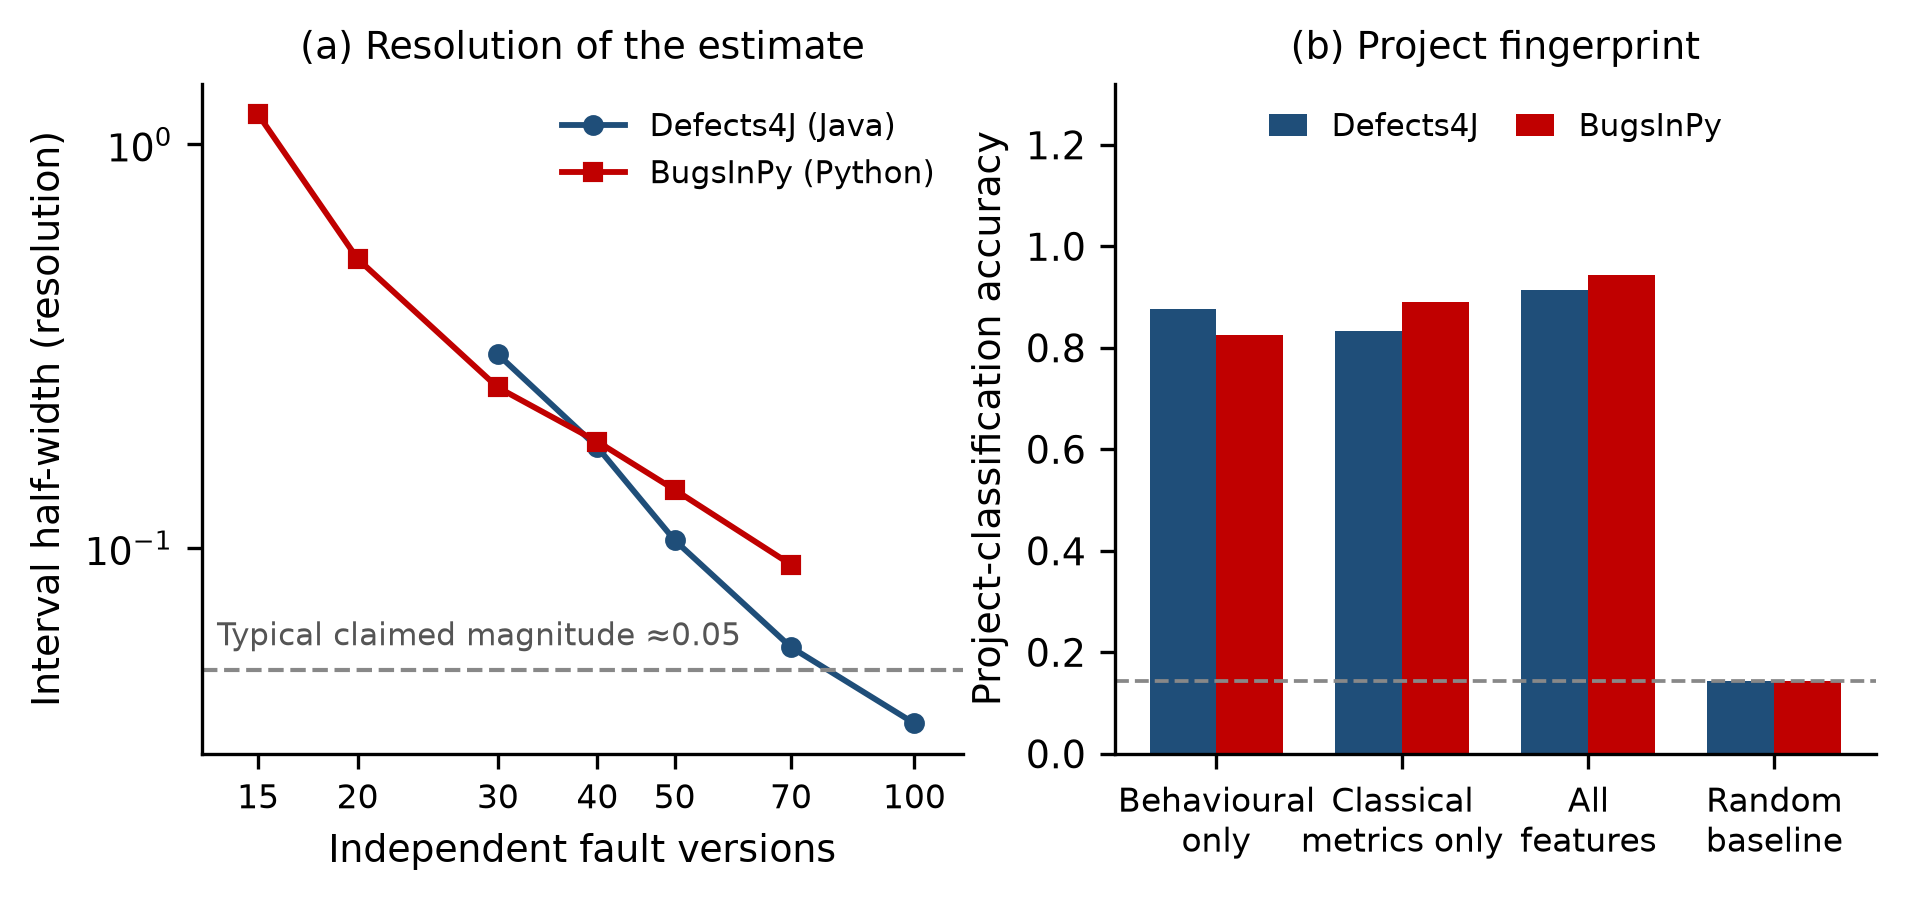
\includegraphics[width=\textwidth]{figures/fig-crossbench-en.png}
\caption{Cross-benchmark comparison. (a) Resolution---the half-width of the 95\% bootstrap interval---against the number of independent fault versions; both benchmarks approach, but do
not reach at conventional sizes, the effect magnitudes typically claimed.
(b) Project-classification accuracy by feature set; both benchmarks exceed the uniform-random-guess baseline by a factor of about six.}
\label{fig:crossbench}
\end{figure*}

\begin{figure*}[t]
\centering
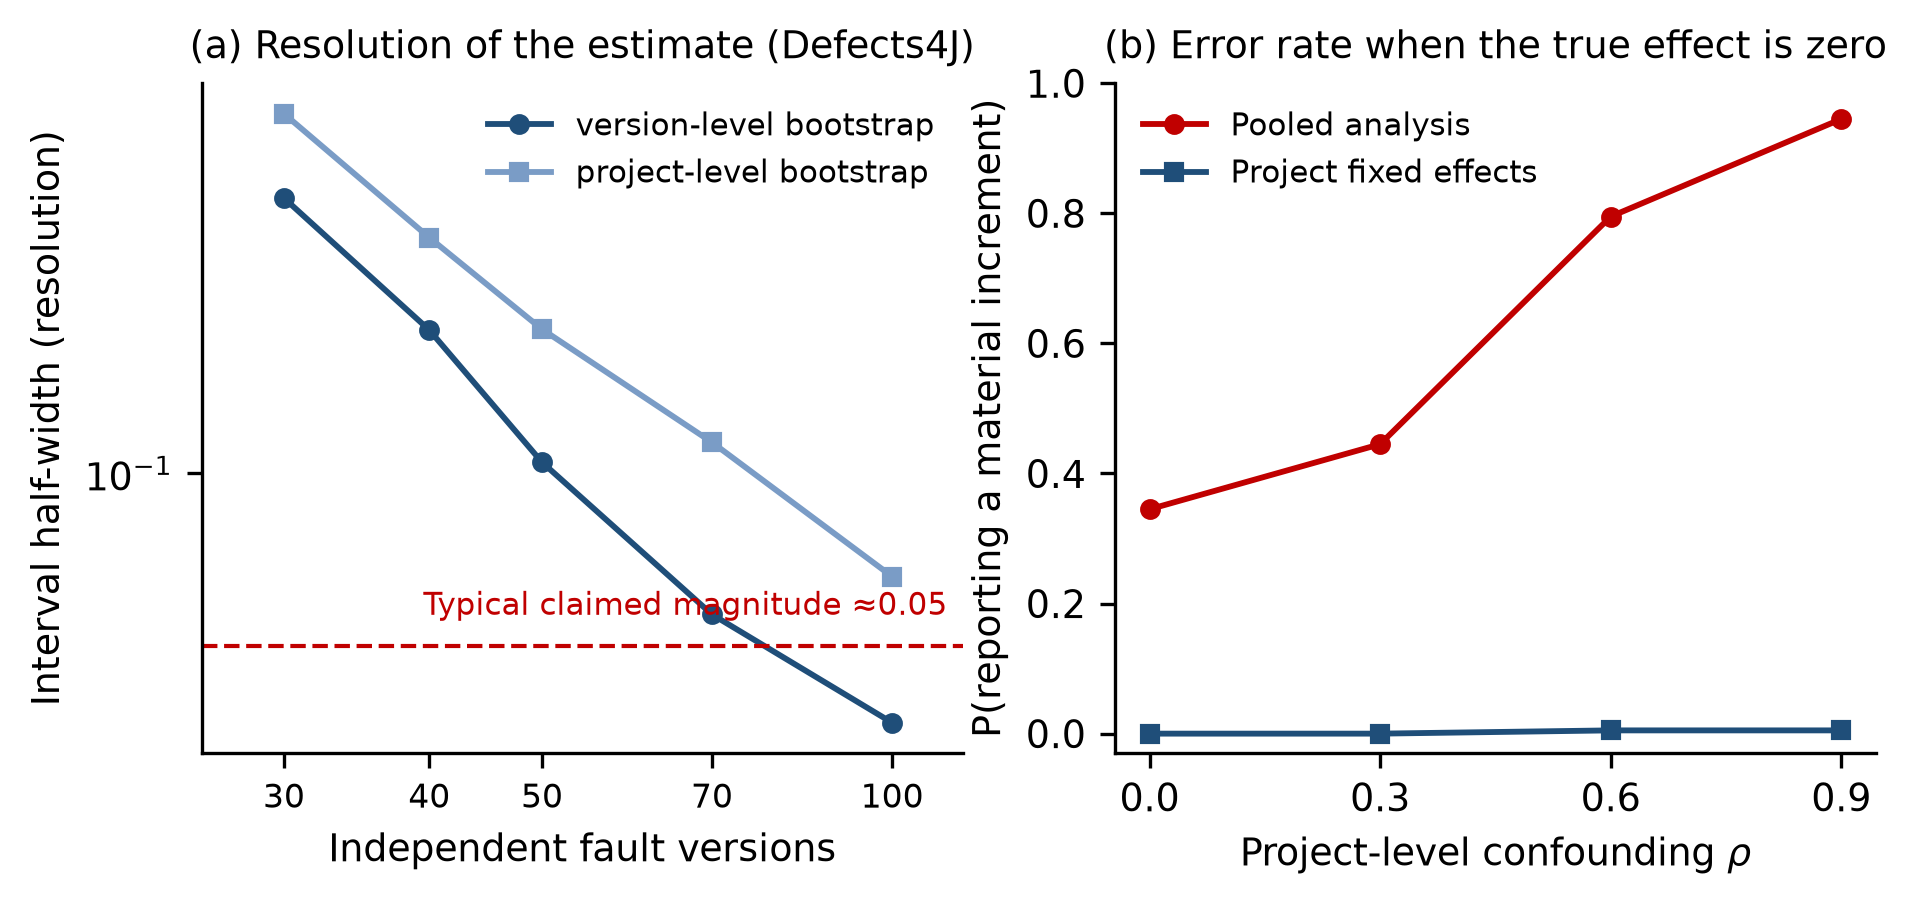
\includegraphics[width=\textwidth]{figures/fig-identifiability-en.png}
\caption{(a) Resolution curve for Defects4J. (b)
Probability of reporting a material increment when the true effect is
zero, as a function of project-level confounding $\rho$; project fixed
effects suppress the artefact.}
\label{fig:identifiability}
\end{figure*}

% =====================================================================
\section{RQ4: How sensitive are the conclusions to analytic choices?}
\label{sec:rq4}

A methodological claim is only useful if it survives the choices a
reasonable analyst might make differently. We test four.

\subsection{Leave-one-project-out}

We recompute the model comparison on each leave-one-project-out sample
(Table~\ref{tab:lopo}).

\begin{table}[t]
\centering
\caption{Leave-one-project-out, with project fixed effects. ``Best'' is the
model with the highest grouped-CV $R^2$ on the reduced sample.}
\label{tab:lopo}
\begin{tabular}{llcc}
\toprule
Benchmark & Project removed & Best model & $\Delta R^2$ \\
\midrule
\multirow{7}{*}{Defects4J}
 & Chart    & Classical & $-0.007$ \\
 & Cli      & Classical & $-0.003$ \\
 & Codec    & Full      & $+0.000$ \\
 & Compress & Classical & $-0.011$ \\
 & Csv      & Classical & $-0.001$ \\
 & Lang     & Classical & $-0.078$ \\
 & Math     & Classical & $-0.007$ \\
\midrule
\multirow{7}{*}{BugsInPy}
 & black      & Full & $+0.037$ \\
 & fastapi    & Full & $+0.017$ \\
 & httpie     & Full & $+0.008$ \\
 & sanic      & Full & $+0.025$ \\
 & tornado    & Full & $+0.017$ \\
 & tqdm       & Size$+$behaviour & $+0.020$ \\
 & youtube-dl & Classical & $-0.019$ \\
\bottomrule
\end{tabular}
\end{table}

On Defects4J the within-project conclusion is stable: six of seven
leave-one-out samples still rank the classical block first, and the
increment stays within $\pm 0.08$ in all seven. On BugsInPy the picture is the
reverse: the full model ranks first in six of seven leave-one-project-out
samples, so the BugsInPy result is not an artefact of pooling alone.
Its magnitude and sign nevertheless remain sensitive to the composition of
projects (Section~\ref{sec:rq4}).

\subsection{Removing the dominant project, and project-size thresholds}

BugsInPy's version counts are highly unbalanced: \texttt{youtube-dl}
contributes 43 of 82 versions. Removing it changes the result materially:
the increment falls from $+0.015$ to $-0.019$ and the best model switches
from full to classical (Table~\ref{tab:subsets}).

\begin{table}[t]
\centering
\caption{Sensitivity to project composition. Cells give the best model
under grouped CV with fixed effects, and the $\Delta R^2$ of the full model
over the classical block.}
\label{tab:subsets}
\begin{tabular}{llccc}
\toprule
Benchmark & Sample & Projects & Best (FE) & $\Delta R^2$ \\
\midrule
\multirow{4}{*}{Defects4J}
 & all            & 7 & Classical & $-0.002$ \\
 & $\geq 2$ versions & 7 & Classical & $-0.002$ \\
 & $\geq 5$ versions & 7 & Classical & $-0.002$ \\
 & $\geq 10$ versions & 4 & Size$+$behaviour & $+0.005$ \\
\midrule
\multirow{3}{*}{BugsInPy}
 & all            & 7 & Full & $+0.015$ \\
 & $\geq 2$ versions & 6 & Full & $+0.025$ \\
 & $\geq 5$ versions & 4 & Full & $+0.045$ \\
 & without \texttt{youtube-dl} & 6 & Classical & $-0.019$ \\
\bottomrule
\end{tabular}
\end{table}

Two honest readings follow. The Defects4J conclusion is robust to
leave-one-project-out perturbations. The BugsInPy conclusion is not robust
to dropping its largest one, and we report this rather than the version
that survives: the cross-language agreement we can claim is that \emph{the
pooled analysis over-states the increment on both benchmarks}, not that the
sign reversal reproduces on both.

Note that the two kinds of perturbation in Table~\ref{tab:subsets} are not
interchangeable. Raising a project-size threshold removes small projects
while retaining the largest, and the BugsInPy increment consequently rises
(from $+0.015$ to $+0.045$) as the sample concentrates on the projects
whose pooled characteristics it was already driven by. Removing the
dominant project does the opposite. The apparent conflict between the
$\geq 5$ and \emph{without youtube-dl} rows is therefore not an
inconsistency but the signature of the same underlying sensitivity: this
benchmark's result is a function of which projects are in it.

\subsection{Bootstrap hierarchy}

The version-level and project-level bootstraps give interval widths of
\num{0.062} and \num{0.129} on Defects4J, and \num{0.143} and \num{0.146}
on BugsInPy (Table~\ref{tab:delta}). The unit of resampling therefore
changes reported uncertainty by a factor of up to two, and the
two hierarchies do not even rank the benchmarks consistently. We report
both throughout rather than choosing the more favourable one, and
recommend that studies state their resampling unit explicitly.

\subsection{Resolution as a design parameter}

The version counts in Table~\ref{tab:mde} are presented as a function of
the target effect rather than as a single number, because the answer
depends on what the study wants to establish. A study aiming to resolve
$\Delta R^2 = 0.10$ is adequately sized at roughly 50 versions; one aiming
at $0.02$ is not adequately sized at any sample this literature typically
reports.

% =====================================================================
\section{A pre-submission protocol}
\label{sec:protocol}

The five checks below are cheap---none requires executing the test suites
under study---and can be applied to any increment-in-$R^2$ claim.

\begin{enumerate}
\item \textbf{Report the nominal sample size and the independent-unit
count.} Compute $n_{\text{nominal}}$, the number of subset instances, and
$n_{\text{ind}} = |\{(\text{project}, \text{version})\}|$, the number of
independent fault-version units. If the ratio is below $0.5$, either
cluster the standard errors or move the analysis to the independent unit.
We deliberately do not call $n_{\text{ind}}$ an ``effective sample size'':
the formal effective sample size of a clustered design also depends on the
within-cluster dependence and on the cluster-size distribution, and we do
not estimate it here. $n_{\text{ind}}$ is a count of independent units, not
a variance-adjusted sample size. Designing for more versions is more
valuable than designing for more subsets per version.
\item \textbf{Screen predictors for project discriminability.} Fit a
classifier predicting project from the predictor block alone. A block whose
accuracy is a large multiple of the baseline ($1/k$ for $k$ projects) will
``predict'' the outcome in any pooled analysis. Report the accuracy.
\item \textbf{Replicate under project fixed effects.} Demean within project
(or add project dummies) and re-fit with standard errors clustered by
version. Report pooled and within-project results side by side; if they
disagree, the disagreement is itself a finding, and the within-project
result is the one to build on.
\item \textbf{State the resampling unit and check the alternative.} Report
whether the bootstrap resamples instances, fault versions, or projects; if
the last is feasible, report it as well, since it reflects the more conservative dependence structure.
\item \textbf{Publish resolution, not just point estimates.} Report the
interval half-width and state the smallest
effect the design could have resolved. If the claimed effect is smaller
than that, the design does not support the claim. Report the required
number of independent fault versions for the target effect, as in
Table~\ref{tab:mde}.
\end{enumerate}

\paragraph{Scope} Fixed effects remove any genuine project-level effect
along with the confounding. Conclusions justified by this protocol are
therefore about \emph{within-project} validity. That is the correct scope
for claims about a metric's diagnostic value for an individual project, but
it must be stated: ``this metric does not help within projects'' and ``this
metric does not help'' are different claims, and only the former follows
from the analysis.

% =====================================================================
\section{Threats to validity}
\label{sec:threats}

\paragraph{Construct validity} The outcome is computed from trigger-test
metadata, which assumes that a suite containing a fault's trigger test
detects that fault. This is the clean-program assumption
\cite{chekam2017empirical}; it makes the outcome cheap and deterministic
but abstracts away from fault masking and oracle quality, so our outcome is
a proxy for detection rather than a direct measurement of it. The
behavioural-matching predictors are syntactic proxies (assertion forms),
not semantic measurements of whether a test asserts intended behaviour; our
conclusions are about the proxy, and they constitute evidence that
syntactic proxies cannot carry the argument---not evidence against the
semantic notion they were meant to index.

\paragraph{Internal validity} Subsets are constructed mechanically at
fractions of the suite, so they vary in composition as well as in size. The
behavioural block and size are correlated in the sample; we control for
$\log$ size in all models, but residual dependence cannot be excluded. On
BugsInPy, coverage is dominated by import-time execution in some projects
(youtube-dl gains only 2 percentage points of coverage between a 10\% and a
60\% subset), which compresses within-project coverage variation and may
understate coverage's within-project value. Finally, the two benchmarks
differ in their classical metric block (BugsInPy has no mutation score), so
the model comparison is not perfectly symmetric across languages.

\paragraph{External validity} Two benchmarks and fourteen projects is a
small basis. Version counts are uneven within BugsInPy (43 down to 1), and
one project contributes over half the Python instances; we report the
leave-one-project-out and dominant-project-removed analyses
(Section~\ref{sec:rq4}) precisely because of this. The extrapolated sample
sizes in Table~\ref{tab:mde} rely on a log--log trend fitted to the
observed curve and should be read as orders of magnitude. The version
counts in Table~\ref{tab:subjects} differ from the number of faults
available in each project; coverage of the benchmark is therefore partial,
and we do not claim it to be exhaustive.

\paragraph{Reliability of the instrument} Both pipelines are our own
implementations. On Defects4J we do not use the framework's test-list
facility (it does not exist); on BugsInPy we do not use the framework's
per-fault checkout (one full clone per fault). Subset construction is
therefore a measurement instrument of our own design, and its fidelity is
supported by targeted checks rather than exhaustive validation. Sample
sizes are reported after dropping records with incomplete metric
measurement; the dropped records are itemised in the replication package.

\paragraph{Statistical conclusions} The bootstrap over seven projects is
itself highly variable, and the project-level intervals in
Table~\ref{tab:delta} should be read with that in mind. The simulation in
Section~\ref{sec:rq2} is a mechanism demonstration with calibrated
dispersion, not an estimate of $\rho$ in either benchmark; the observed
project-level correlation in our Defects4J sample is weak
($\rho \approx -0.07$ across seven projects, itself imprecisely estimated),
so the $\rho$ sweep should be read as ``if $\rho$ were $x$'' rather than as
a description of these benchmarks.

% =====================================================================
\section{Conclusion}
\label{sec:conclusion}

A common design for validating test-adequacy metrics is incremental
prediction. We have shown, on two independent benchmarks in two
languages, that this instrument is not sharp enough for the conclusions
typically drawn from it: the effects being claimed are of the same order as
the uncertainty of their own estimates, their sign depends on unreported
analyst choices, and project-level confounding alone can produce them in up to 94\% of
runs.

None of this implies that test-adequacy metrics are worthless, or that the
existing studies are dishonest. It implies that the field's reporting
convention---a point estimate and a $p$-value---does not carry the
information readers need in order to judge the claim. The protocol in
Section~\ref{sec:protocol} is offered as a minimal remedy: five checks that
cost no test executions, and a resolution statement that tells the reader
what the study could have found.

\section*{Data and code availability}

All scripts, collected measurements, and analysis code are available at
\url{https://github.com/JunjieChen0/test-adequacy-resolution}.
Every number reported in this paper is produced by
\texttt{scripts/analyze\_all.py} from the shipped measurements; the
repository contains both benchmarks' per-instance records, the analysis
outputs, and a step-by-step reproduction guide.

\bibliographystyle{elsarticle-num}
\bibliography{refs}

\end{document}
